\begin{ex}
	Với $a, b$ là hai số thực dương tùy ý, $\log _{3}\left(a b^{3}\right)$ bằng
	\choice
	{$\log _{3} a+\frac{1}{3} \log _{3} b$}
	{$ 3\left(\log _{3} a+\log _{3} b\right)$}
	{\True $ \log _{3} a+3 \log _{3} b$}
	{$3 \log _{3} a+\log _{3} b $}
\end{ex}

\begin{ex}
\immini[thm]{Cho hàm số $y=f(x)$ có đồ thị như hình vẽ. Số điểm cực trị của hàm số là
\choice[1]
{$0$}
{$1$}
{\True $3$}
{$2$}
}{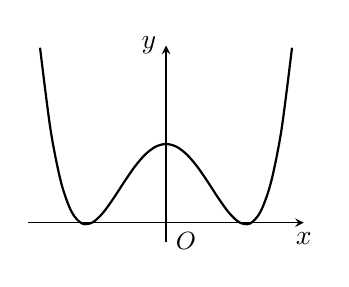
\begin{tikzpicture}[scale=.5]
\draw[-stealth] (-3.5,0) -- (3.5,0) node[below]{$x$};
\draw[-stealth] (0,-0.5) -- (0,4.5) node[left]{$y$};
\draw (0,0) node[below right]{\small $O$};
\draw[thick,smooth] plot[domain=-3.2:3.2](\x,{0.12*(\x)^4-.99*(\x)^2+2});
\end{tikzpicture}}
\end{ex}

\begin{ex}
Cho mặt cầu có diện tích bằng $16 \pi \mathrm{cm}^{2}$. Bán kính của mặt cầu đó bằng
\choice
{\True$ 2 \mathrm{~cm}$}
{$2 \sqrt{3} \mathrm{~cm}$}
{$4 \mathrm{~cm}$}
{$\sqrt[3]{12} \mathrm{~cm}$}
\end{ex}

\begin{ex}
Tập xác định của hàm số $y=\left(x^{3}-27\right)^{\frac{\pi}{4}}$ là
\choice
{$\mathscr{D}=\mathbb{R} \backslash\{3\}$}
{\True$ \mathscr{D}=(3 ;+\infty)$}
{$\mathscr{D}=[3 ;+\infty)$}
{$\mathscr{D}=\mathbb{R}$}
\end{ex}

\begin{ex}
Diện tích xung quanh của hình nón có bán kính đáy $r=4$ và độ dài đường sinh $l=5$ bằng
\choice
{$40 \pi$}
{$16 \pi$}
{$12 \pi$}
{\True$ 20 \pi$}
\end{ex}

\begin{ex}
Thể tích khối lăng trụ có diện tích đáy $B=6$ và chiều cao $h=7$ bằng
\choice
{\True 42}
{32}
{14}
{24}
\end{ex}

\begin{ex}
Tiệm cận đứng của đồ thị của hàm số $y=\dfrac{x+2}{-2 x+1}$ có phương trình
\choice
{$x=-\dfrac{1}{2}$}
{$x=2$}
{\True$ x=\dfrac{1}{2}$}
{$x=-2$}
\end{ex}
\begin{ex}
Cho số phức $z=-3+5i$. Phần ảo của số phức $z$ bằng
\choice
{$5i$}
{\True $5$}
{$3$}
{$-3$}
\end{ex}
\begin{ex}
Tọa độ điểm cực đại của đồ thị hàm số $y=x^{3}-3 x^{2}+2$ là
\choice
{$(0 ;-2)$}
{$(2 ;-2)$}
{\True $(0 ; 2)$}
{$(2 ; 2)$}
\end{ex}